\documentclass{beamer}

% latex commands and macros

% common sets
\newcommand{\R}{\mathbb{R}} % the set of real numbers
\newcommand{\C}{\mathbb{C}} % the set of complex numbers
\newcommand{\Z}{\mathbb{Z}} % the set of integers
\newcommand{\N}{\mathbb{N}} % the set of natural numbers
\newcommand{\Q}{\mathbb{Q}} % the set of rational numbers
\newcommand{\F}{\mathbb{F}} % usually stands for field
\newcommand{\D}{\mathbb{D}} % the unit disc in the complex plane
\newcommand{\B}{\mathbb{B}} % the unit ball
\newcommand{\es}{\mathbb{S}} % sphere
\newcommand{\T}{\mathbb{T}} % torus
\newcommand{\RP}{\mathbb{R}P} % projective plane
\newcommand{\CP}{\mathbb{C}P} % complex projective plane
\DeclareMathOperator \Gr {Gr} % grassmannian
\newcommand{\ham}{\mathbb{H}} % quaternions

% common operations and connectors
\newcommand{\inner}[2]{\left<{#1},\,{#2}\right>} % inner product
\newcommand{\coset}[1]{\left<{#1}\right>} % groups or ideal generated by some set
\newcommand{\norm}[1]{\left\|{#1}\right\|} % norm of a vector
\newcommand{\abs}[1]{\left|{#1}\right|} % absolute value
\newcommand{\sets}[1]{\left\{{#1}\right\}} % a simple set with no conditions
\newcommand{\set}[2]{\sets{{#1}:\,{#2}}} % a set with conditions
\newcommand{\prn}[1]{\left({#1}\right)} % parentheses 
\newcommand{\brak}[2]{\left[{#1},\,{#2}\right]} % bracket product
\newcommand{\pbrak}[2]{\left\{{#1},{#2}\right\}} % Poisson bracket product

\DeclareMathOperator \csum {\#} % connected sum

\DeclareMathOperator \pp {\,a.e.} % almost everywhere
\DeclareMathOperator \sgn {sgn} % signum function
\DeclareMathOperator \spn {span} % span
\DeclareMathOperator \cspn {\overline{span}} % closed span
\DeclareMathOperator \img {Im} % imaginary part of a complex number
\DeclareMathOperator \rea {Re} % real part of a complex number
\DeclareMathOperator \ind {ind} % index of a function
\DeclareMathOperator \diam {diam} % diameter of a set or a graph
\DeclareMathOperator \res {res} % residue of a complex function
\DeclareMathOperator \dist {dist} % distance function
\DeclareMathOperator \wind {wind} % winding number
\DeclareMathOperator \spectrum {\sigma} % spectrum of an operator
\DeclareMathOperator \spectrumEssential {\sigma_{\text{ess}}} % essential spectrum of an operator

\DeclareMathOperator \smb {smb} % symbol $C^*$-homomorphism

\newcommand{\acton}[2]{\phantom{|}^{{#1}}{{#2}}} % hack to prepend a superscript

\DeclareMathOperator \Syl {Syl} % Sylow subgroup
\DeclareMathOperator \im {im} % image of a function
\DeclareMathOperator \Tor {Tor} % torsion
\DeclareMathOperator \Aut {Aut} % automorphisms
\DeclareMathOperator \End {End} % endomorphisms
\DeclareMathOperator \Mod {Mod} % modules
\DeclareMathOperator \Hol {Hol} % holomorphic functions
\DeclareMathOperator \Sym {Sym} % symmetric group
\DeclareMathOperator \Alt {Alt} % alternating groups
\DeclareMathOperator \Mat {Mat} % matrices
\DeclareMathOperator \Spec {Spec} % spectrum of a ring
\DeclareMathOperator \Max {Max} % maximal spectrum of a ring
\DeclareMathOperator \coker {coker} % cokernel
\DeclareMathOperator \GL {GL} % general linear group
\DeclareMathOperator \SL {SL} % special linear group
\DeclareMathOperator \codim {codim} % codimension of a vector subspace
\DeclareMathOperator \rnk {rnk} % rank of a linear transform
\DeclareMathOperator \Id {Id} % identity function
\DeclareMathOperator \Tr {Tr} % trace of a matrix
\DeclareMathOperator \diag {diag} % diagonal matrix
\DeclareMathOperator \supp {supp} % support of a function

% category theory
\DeclareMathOperator \Ob {Ob} % objects
\DeclareMathOperator \Mor {Mor} % morphism
\DeclareMathOperator \Hom {Hom} % homomorphisms
\DeclareMathOperator \Lin {\mathbf{Lin}} % linear
\DeclareMathOperator \Set {\mathbf{Set}} % sets
\DeclareMathOperator \Vect {\mathbf{Vect}} % vector spaces

% vector calculus
\DeclareMathOperator \diver {div} % divergence
\DeclareMathOperator \grad {grad} % gradient
\DeclareMathOperator \curl {curl} % curl

\DeclareMathOperator \Lie {Lie} % Lie groups
\newcommand{\lie}[1]{\mathfrak{{#1}}} % lie algebra

% operator analysis
\newcommand \slim {\text{s-}\lim} % strong limit
\DeclareMathOperator \Fl{\mathbb{F}l} % spaces of frequency weighted norms
\DeclareMathOperator \Smb{Smb} % symbol operator
\DeclareMathOperator \Alg{Alg} % algebra generated by a set

% statistics
\DeclareMathOperator \Exp{\mathbb{E}} % variance
\DeclareMathOperator \Var{Var} % variance

% miscellaneous

% frequently used abbreviations
\newcommand{\ve}{\varepsilon} % epsilon clearly distinguishable from inclusion
\newcommand{\vf}{\varphi} % more popular way of writing phi
\newcommand{\vn}{\varnothing} % the empty set

% special notation for dissertation
\newcommand{\hprod}{\circ} % Hadamard or entrywise multiplication of matrices
\newcommand{\hs}{{\mathcal{C}_2}} % Hilbert-Schmidt class
\newcommand{\poi}{{\mathcal{P}_1}} % Poincare class
\newcommand{\MellinTransform}{\mathcal{M}} % Mellin Transform
\newcommand{\MellinConvolution}{*_{\MellinTransform}} % Mellin convolution

% environments and fonts for cifar-ten project
\newcommand{\code}[1]{\texttt{{#1}}}

% styles of theorems, definitions and remarks
\theoremstyle{plain}
\newtheorem{thm}{Theorem}%[section]
\newtheorem{lemma}[thm]{Lemma}
\newtheorem{prop}[thm]{Proposition}
\newtheorem{cor}[thm]{Corollary}
\newtheorem{axiom}[thm]{Axiom}
\newtheorem{exercise}[thm]{Exercise}
\newtheorem{claim}[thm]{Claim}
\newtheorem{fact}[thm]{Fact}

\theoremstyle{definition}
\newtheorem{defn}[thm]{Definition}

\theoremstyle{remark}
\newtheorem{remark}[thm]{Remark}
\newtheorem{exmpl}[thm]{Example}
\newtheorem{problem}[thm]{Problem}
\newtheorem{prob}[thm]{Problem}
\newtheorem{fle}[thm]{File}

% page format
\oddsidemargin=0in
\evensidemargin=0in
\textwidth=6in
\topmargin=-0.5in
\textheight=9.5in
\parindent=.375in

% packages
\usepackage{enumerate}
\usepackage{amssymb}
%\usepackage[all,cmtip]{xy}
\usepackage[mathscr]{eucal}
\usepackage{graphicx,color}

\newcommand{\titleChaos}[1]{\title[HW {#1}]{Introduction to Chaos, Homework {#1}}}

%\begin{figure}[ht]
%       \includegraphics[height=1in,keepaspectratio]{03NegativeHelix.jpg}
%       \caption{Negative writhe crossings} \label{fig:negativeWritheCrossings}
%\end{figure}


% packages
\usepackage{beamerthemesplit}
\usepackage{enumerate}
\usepackage{amssymb}
\usepackage[all,cmtip]{xy}
\usepackage[mathscr]{eucal}
\usepackage[natbib=true,style=authoryear,backend=bibtex,useprefix=true]{biblatex}
\addbibresource{reading.bib}
\usepackage{graphicx,color}

\title{RL}
\author{Reuben Brasher}
\date{\today}

\begin{document}

\frame{\titlepage}

\section[Outline]{}
\frame{\tableofcontents}

\section{Pictures of games}

\frame
{
   \frametitle{N-Armed Bandit}
   
   Refer to Fig. \ref{fig:narmed}.
   
   \begin{figure}[ht]
      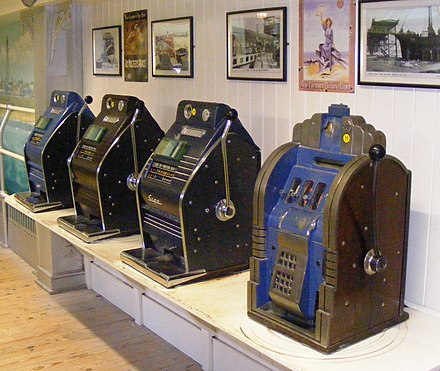
\includegraphics[height=2in,keepaspectratio]{images/Slot_machines_at_Wookey_Hole_Caves.JPG}
      \caption{https://search.creativecommons.org/photos/70ab8654-c234-4dbe-9b1c-62851544245a} \label{fig:narmed}
   \end{figure}
}

\frame
{
   \frametitle{Markov Decision Process}
   
   Refer to Fig. \ref{fig:mdp}.
   
   \begin{figure}[ht]
      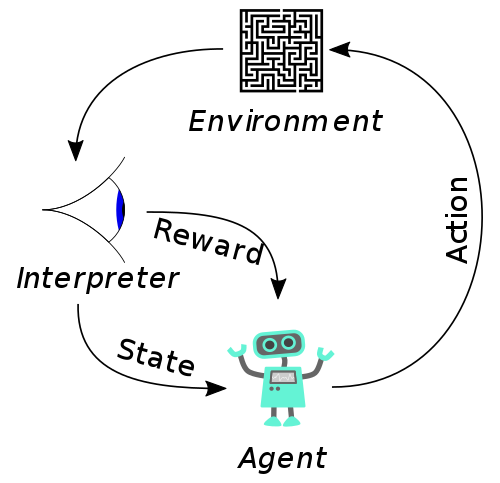
\includegraphics[height=2in,keepaspectratio]{images/Reinforcement_learning_diagram.svg.png}
      \caption{https://search.creativecommons.org/photos/70ab8654-c234-4dbe-9b1c-62851544245a} \label{fig:mdp}
   \end{figure}
}

\frame
{
   \frametitle{LSTM and GRU}

   ``Long short-term memory''\cite{hochreiter1997long}

   ``Empirical evaluation of gated recurrent neural networks on sequence modeling''\cite{chung2014empirical}
}

\frame
{
   \frametitle{LSTM and GRU secret sauce}

   \begin{itemize}
      \item<1-> Entrywise multiplication of two previous layers outputs

      $$(x \odot y)_i = x_i y_i$$

      \item<2-> Called gates because they are conintuous analogs of boolean and gates. If $x$ and $y$ are strictly 1 or 0, then
      
      $$x \wedge y = x \times y$$

   \end{itemize}
}


\frame
{
   \frametitle{LSTM suggestive names}

   \begin{itemize}
      \item<1-> Activation, $h^j_t = o^j_t \tanh \prn{c^j_t}$.
      
      \item<2-> Output gate, $o^j_t = \sigma \prn{ \prn{W_o x_t + U_o h_{t-1} + V_o c_t}^j }$

      \item<3-> Memory cell, $c^j_t = f^j_t c^j_{t-1} + i^j_t \tilde c^j_t$

      \item<4-> Memory content, $\tilde c^j_t = \tanh \prn{ \prn{W_c x_t + U_c h_{t-1}}^j }$

      \item<5-> Forget gate, $f^j_t = \sigma \prn{W_f x_t + U_f h_{t-1} + V_f c_{t-1}}$

      \item<6-> Input gate, $i^j_t = \sigma \prn{W_i x_t + U_i h_{t-1} V_i c_{t-1}}$

   \end{itemize}
}

\frame
{
   \frametitle{LSTM rewritten}

   \begin{itemize}
      \item<1-> Activation, $h_t = o_t \odot \tanh \prn{c_t}$.
      
      \item<2-> Output gate, $o_t = \sigma \prn{A_o \prn{x_t, h_{t-1}, c_t}}$

      \item<3-> Memory cell, $c_t = f_t \odot c_{t-1} + i_t \odot \tilde c_t$

      \item<4-> Memory content, $\tilde c_t = \tanh \prn{A_c \prn {x_t, h_{t-1}}}$

      \item<5-> Forget gate, $f_t = \sigma \prn{ A_f \prn{x_t, h_{t-1}, c_{t-1}}}$

      \item<6-> Input gate, $i_t = \sigma \prn{ A_i \prn{x_t, h_{t-1}, c_{t-1}}}$

   \end{itemize}
}

\frame
{
   \frametitle{GRU suggestive names}

   \begin{itemize}
      \item<1-> Activation, $h_t = \prn{1 - z_t} \odot h_{t-1} + z_t \odot \tilde h_t$.
      
      \item<2-> Update gate, $z_t = \sigma \prn{A_z \prn{x_t, h_{t-1}}}$

      \item<3-> Candidate activations, $\tilde h_t = \tanh \prn{A \prn{x, r \odot h_{t-1}}}$

      \item<4-> Reset gate, $r_t = \sigma \prn{A_r \prn{x_t, h_{t-1}}}$

   \end{itemize}
}

\section{RNN with attention}

\frame
{
   \frametitle{Sequence to sequence with attention}

   % image

   ``Neural machine translation by jointly learning to align and translate'' \cite{bahdanau2014neural}
}

\frame
{
   \frametitle{Attention Layers}

   \begin{itemize}
      \item<1-> Let $x_j$ be the input sequence and $h_j$ encoding by RNN.

      \item<2-> Let $y_i$ be the target sequence, and $s_i$ a hidden state.

      \item<3-> $$s_i = f \prn{s_{i-1}, y_{i-1}, c_i}$$

      \item<4-> $c_i$, called the context vector is

      $$c_i = \sum_j \alpha_{ij} h_j$$

      \item<5-> $\alpha_{ij}$ is the importance of $h_j$ for $s_i$

      $$\alpha_{ij} = \frac{\exp \prn{e_{ij}}} {\sum_k \exp \prn{e_{ik}}}$$

      where $e_{ij} = a \prn{a_{i-1}, h_j}$.

      
   \end{itemize}
}

\begin{frame}[t,allowframebreaks]
   \frametitle{References}
   \printbibliography
\end{frame}

\end{document}
